\documentclass[tikz,border=10pt]{standalone}
\usetikzlibrary{shapes.geometric, arrows}

\tikzstyle{startstop} = [rectangle, rounded corners, minimum width=3cm, minimum height=1cm,text centered, draw=black, fill=orange!30]
\tikzstyle{process} = [rectangle, minimum width=3cm, minimum height=1cm, text centered, draw=black, fill=orange!30]
\tikzstyle{decision} = [diamond, minimum width=3cm, minimum height=1cm, text centered, draw=black, fill=green!30]
\tikzstyle{arrow} = [thick,->,>=stealth]
\tikzstyle{io} = [trapezium, trapezium left angle=70, trapezium right angle=110, minimum width=3cm, minimum height=1cm, text centered, draw=black, fill=blue!30]

\begin{document}

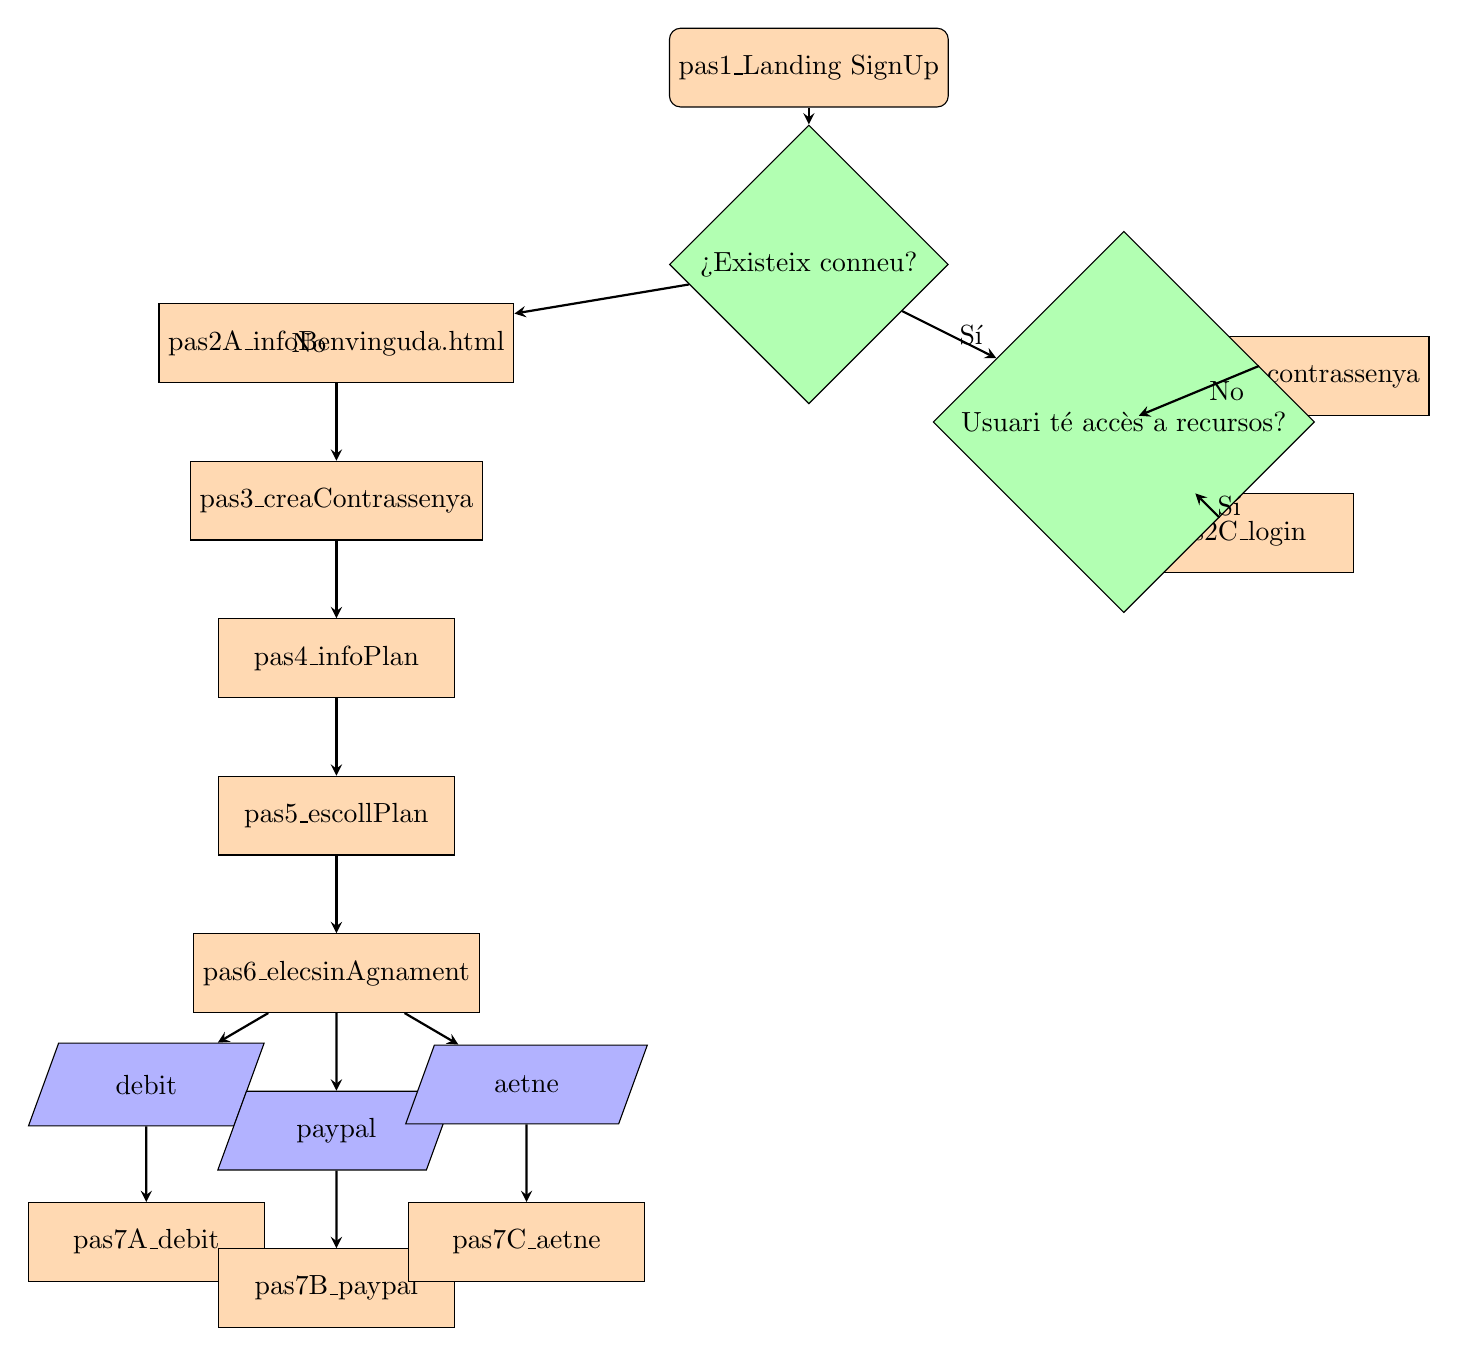
\begin{tikzpicture}[node distance=2cm]

\node (start) [startstop] {pas1\_Landing SignUp};
\node (dec1) [decision, below of=start, yshift=-0.5cm] {¿Existeix conneu?};
\node (pas2a) [process, left of=dec1, xshift=-4cm, yshift=-1cm] {pas2A\_infoBenvinguda.html};
\node (pas3) [process, below of=pas2a] {pas3\_creaContrassenya};
\node (pas4) [process, below of=pas3] {pas4\_infoPlan};
\node (pas5) [process, below of=pas4] {pas5\_escollPlan};
\node (pas6) [process, below of=pas5] {pas6\_elecsinAgnament};
\node (debit) [io, below left of=pas6, xshift=-1cm] {debit};
\node (paypal) [io, below of=pas6, xshift=0cm] {paypal};
\node (aetne) [io, below right of=pas6, xshift=1cm] {aetne};
\node (pas7a) [process, below of=debit] {pas7A\_debit};
\node (pas7b) [process, below of=paypal] {pas7B\_paypal};
\node (pas7c) [process, below of=aetne] {pas7C\_aetne};

\node (pas2b) [process, below right of=dec1, xshift=4cm] {pas2B\_introdueix contrassenya};
\node (pas2c) [process, below of=pas2b] {pas2C\_login};

\node (dec2) [decision, below of=dec1, xshift=4cm] {Usuari té accès a recursos?};

% Arrows
\draw [arrow] (start) -- (dec1);
\draw [arrow] (dec1) -- (pas2a)  node[anchor=east] {No};
\draw [arrow] (pas2a) -- (pas3);
\draw [arrow] (pas3) -- (pas4);
\draw [arrow] (pas4) -- (pas5);
\draw [arrow] (pas5) -- (pas6);
\draw [arrow] (pas6) -- (debit);
\draw [arrow] (pas6) -- (paypal);
\draw [arrow] (pas6) -- (aetne);
\draw [arrow] (debit) -- (pas7a);
\draw [arrow] (paypal) -- (pas7b);
\draw [arrow] (aetne) -- (pas7c);

\draw [arrow] (dec1) -- node[anchor=west] {Sí} (dec2);
\draw [arrow] (dec2) -- node[anchor=west] {No} (pas2b);
\draw [arrow] (dec2) -- node[anchor=west] {Sí} (pas2c);

\end{tikzpicture}

\end{document}
